\chapter{Návrh riešenia} \label{chapter:design}
V súlade so stanovenými kritériami navrhneme postupnosť krokov úpravy nameraného pohybu dopravného prostriedku.
Zhotovenú konfigurovateľnú sústavu uplatníme na zariadení senzorovej jednotky za účelom ohlasovania udalostí
o vybraných pravidelných rysoch signálu. Prihliadať sa bude viac na rýchlu odozvu splnenia úloh pri
dosiahnuteľnom výkone v dostupnom pamäťovom priestore, ako na energetickú úsporu. Výmena údajov sa má
odohrávať širko podporovaným formátom za redukcie nadbytočného sieťového prenosu.

\section{Špecifikácia požiadaviek}
Zariadenie internetu vecí určené na analýzu vibrácií z prostredia bude realizovať nasledujúce funkcionálne požiadavky:
\begin{itemize}[noitemsep,topsep=0pt]
\item Zber trojosovej akcelerácie s nastaviteľnou vzorkovacou frekvenciou a dynamickým rozsahom akcelerometra, v hraniciach danými
obmedzeniami hardvéru, najmenej však intenzity vyskytujúcej sa pri preprave konvenčnými pozemnými motorovými vozidlami.
\item Spracovanie osí akcelerácie nezávisle s obmedzením výberu aktívnych osí.
\item Vzdialene realizovateľná zmena parametrov jednotlivých stupňov sústavy na úpravu akceleračného signálu v posuvných oknách.
\item Ukladanie nameranej akcelerácie na pamäťovú kartu s ohľadom na najvyššiu dosiahnuteľnú rýchlosť zápisu.
\item Identifikácia významných frekvencií so zachytením ich trvania a amplitúdy podľa aktuálnej
konfigurácie detekčných algoritmov.
\item Notifikácia detegovanej udalosti o zmene vibračného spektra bude odoslaná bezdrôtovou sieťovou linkou do 10 sekúnd od objavenia.
\item Sumarizácia hodnôt akcelerácie po posuvných oknách do popisných štatistík.
\item Odosielanie zachytených udalostí cez spoľahlivé sieťové spojenie za dosiahnutia redukcie množstva produkovaných dát.
\item Poskytnutie možnosti odosielania výsledkov z podstatných medzikrokov spracovania za účelom ich poskytnutia
ďalším úrovniam senzorovej siete alebo na skupinovú koordináciu meraní z viacerých uzlov.
\item Výmena údajov cez sieťový protokol v štandardizovanom formáte hierarchickej štruktúry za najmenšej uskutočniteľnej réžie.
\end{itemize}
\bigskip

Z povahy okolností nasadenia firmvéru na relatívne zdrojovo oklieštené Edge zariadenie vyplývajú
vymenované nefunkcionálne požiadavky, prevažne na účinnosť a prenositeľnosť:
\begin{itemize}[noitemsep,topsep=0pt]
\item Firmvér sa zmestí do programovej pamäte s rezervou pre budúce rozširovanie detekčnej funkcionality.
\item Ľubovoľný scenár spracovania musí prebehnúť v reálnom čase rádovo v jednotkách sekúnd.
\item Platformová závislosť sa obmedzí na nevyhnutné súčasti systému ako sú hardvérové ovládače a akcelerácia náročných výpočtov.
\end{itemize}

\section{Hardvér senzorovej jednotky}
Navrhované zariadenie je postavené na platforme mikrokontroléra ESP32 od Espressif. Za relatívne nízkej obstarávacej ceny
ponúka možnosť konektivity na 2,4 GHz s Wifi 802.11 b/g/n a Bluetooth 4.2. V porovnaní s podobnými zariadeniami disponuje
nebývalým výpočtovým výkonom a kapacitou pamätí. Univerzálny plošný spoj osadený kontrolérom a neskôr zmienenými
komponentami je zabezpečený externým zhotoviteľom.

Konkrétne je systém postavený na doske FireBeetle osadenej modulom ESP32-WROOM-32D s typickým napájacím napätím 3,3 V a dvoj-jadrovým
32-bitovým procesorom Xtensa s taktovacou frekvenciou od 80 do 240 MHz. Modul obsahuje až 520 kB SRAM logicky rozdelenej
na 192 kB IRAM časť pre inštrukcie a 328 kB DRAM na dáta.

Použitý model akcelerometera je súčasťou MEMS inerciálnej meracej jednotky LSM9DS1 (pozri \ref{section:accelometers}),
zabudovanej na adaptéri STEVAL-MKI159V1 pre púzdro DIL24. Akcelerometer komunikuje s MCU cez
poloduplexnú SPI zbernicu s maximálnou frekvenciou hodín do 10 MHz. Navyše sa zapoja vývody prerušení INT1 a INT2
pre upozornenie prekročenia určených prahových úrovní. Blokový diagram zapojenia zachytáva schéma \ref{schematics:block}.

\begin{figure}[h]
\centering
\begin{subfigure}[b]{0.65\textwidth}
    \centering
    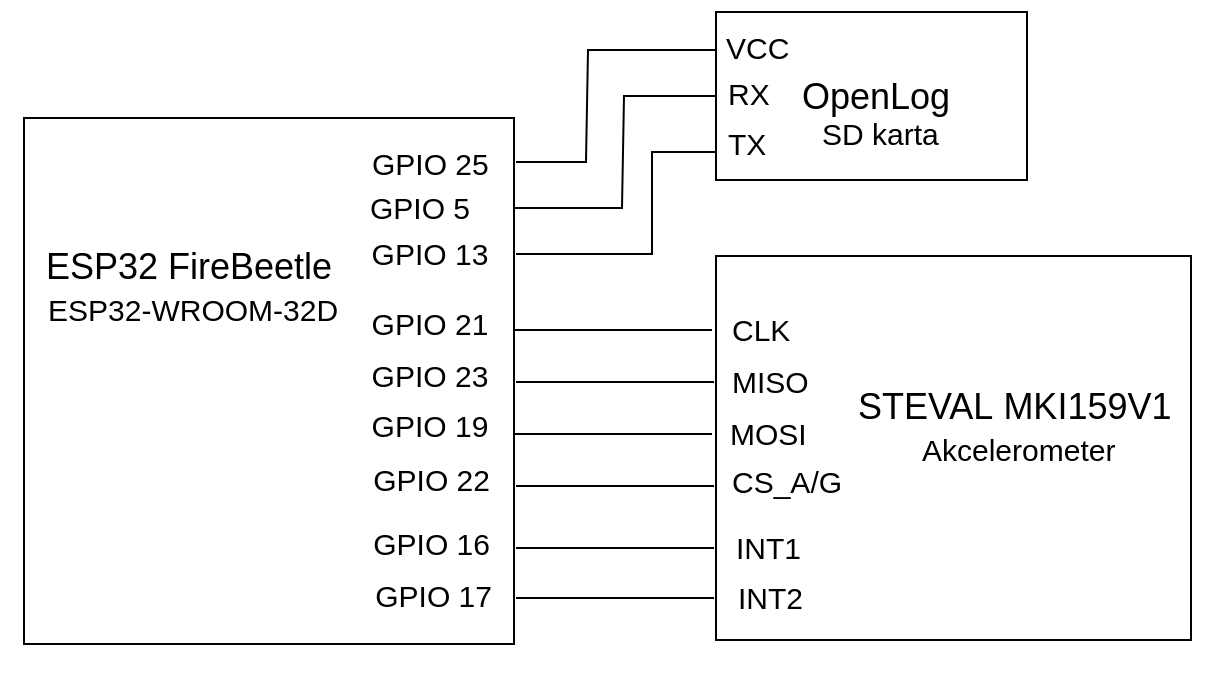
\includegraphics[width=\textwidth]{figures/design/block-circuit-diagram.png}
    \caption{Blokový diagram modulov}
       \label{schematics:block}
\end{subfigure}
\hfill
\begin{subfigure}[b]{0.3\textwidth}
    \centering
    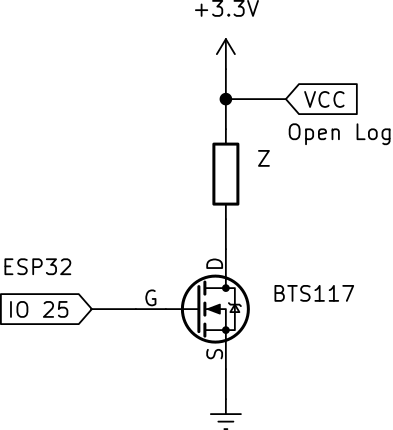
\includegraphics[width=\textwidth]{figures/design/fet.png}
    \caption{Ovládanie napájania OpenLog cez FET}
    \label{schematics:fet}
\end{subfigure}
\label{schematics}
\caption{Schéma zapojenia hardvéru}
\end{figure}

Pamäťová Micro SD karta so súborovým systémom FAT32 bude pripojená v module OpenLog od Sparkfun, ktorý zaznamená znaky
prijímané cez UART do textových súborov podľa pravidiel zo súboru \verb|config.txt| alebo povelmi odoslanými
po zapnutí. Ukladanie na externé médium nie je vždy žiaduce, preto bude napájanie spínané cez pin mikrokontroléra. Vyšší
prúdový odber než dodá výstup a požadované napätie rovné s napájacím napätím procesora vyžaduje umiestnenie tranzistora riadeného
poľom N-kanál BTS117 na premostenie riadiaceho signálu (obr. \ref{schematics:fet}).


\section{Architektúra systému}
Celková skladba komponentov systému (\ref{uml:component}) pozostáva zo súčastí pôsobiacich na mikrokontroléri ESP32
interagujúcimi cez lokálne sériové zbernice s akcelerometrom a zapisovačom. Spracované vektory akcelerácie sú
odosielané do počítačovej siete prostredníctvom prístupového bodu WiFi aplikačným protokolom MQTT
na server so službou broker správ. Odoberané témy sú odtiaľ rozšírené klientom metódou publish-subcribe.
\begin{figure}[h]
	\centering
	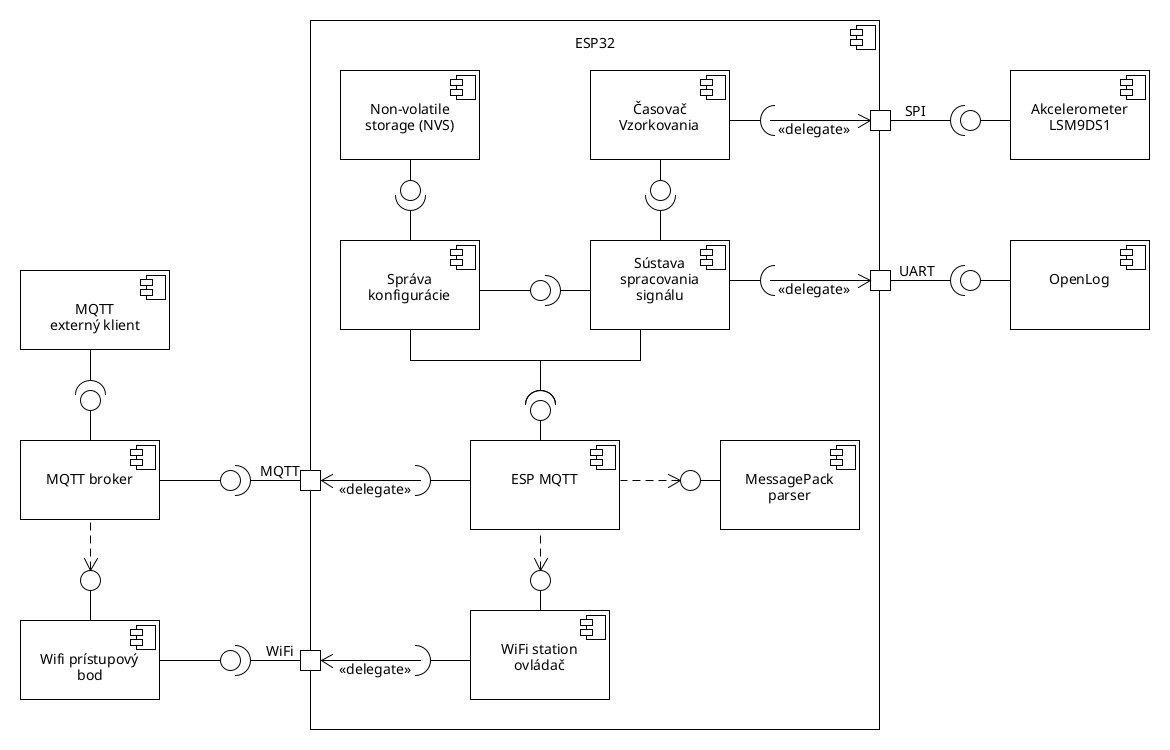
\includegraphics[width=\textwidth]{figures/design/components.png}
	\caption{Komponenty navrhovaného systému}
	\label{uml:component}
\end{figure}

Odčítavanie úrovní z akcelerometra zabezpečuje \textbf{časovač vzorkovania}, ktorý si v pravidelných intervaloch pýta aktuálne
hodnoty rozhraním periférneho adaptéra pre prístup ku SPI zbernici. Po vypršaní vzorkovacej periódy je zavolaná obsluha prerušenia, ktorá
odblokuje vlákno úlohy na synchrónne načítanie okamžitého vektora zrýchlenia konvertovaného z číslicovej úrovne prevodníka na metre za
sekundu na druhú (\ref{uml:sequence}). Zachytené hodnoty sú preposlané cez thread-safe rady analyzátora signálu zvlásť pre každú
priestorovú os akcelerácie. V prípade zachytávania časového priebehu s voliteľným podvzorkovaním sa vektor umiestni do radu pre
vlákno loggera.

\textbf{Sústava spracovania signálu} (\ref{uml:component}) rozdeľuje vzorky do prelínajúcich sa posuvných okien, počíta z nich štatistiky
a vyhľadáva udalosti vo frekvenčnom spektre. Nespracované hodnoty sú podľa potreby ukladané na pamäťovú kartu.

\textbf{Správa konfigurácie} zaobstaráva zmenu a uchovanie parametrov pipelinov pre jednotlivé bloky spracovania.
Modifikované nastavenia sú
medzi spusteniami zachované vo vyhradenej partícií nevolatilnej flash pamäte na záznamy dvojíc v asociatívnej štruktúre. Predvolené
správanie načítané za nedostupnosti konfigurácie z flash úložiska určujú konštanty v programovej pamäti.

Binárny serializačný formát Message Pack zaobaľuje vzorky, udalosti a konfiguráciu posielané na rozličné MQTT témy. Vychádza z
formátu JSON (JavaScript Object Notation), ale na rozdiel od neho sa sústredí na efektívne kódovanie dátových typov. Namiesto prevodu
číselných údajov do znakového kódovania, napr. Unicode, ponecháva ich pôvodnú binárnu reprezentáciu so štandardom špecifikovanými bytovými
značkami určujúcimi typ údaju. Hodnoty vyjadriteľné menším počtom bajtov reprezentuje dokonca v kratšom tvare než
podmieňuje ich celkový rozsah. V zoznamoch a slovníkov sa zaobchádza bez oddelovacích znakov, ktoré nahrádza
informáciou o počte údajov. Dĺžka položky predchádzajúca zloženými atribútom uľahčuje následné parsovanie.

\begin{figure}[h]
	\centering
	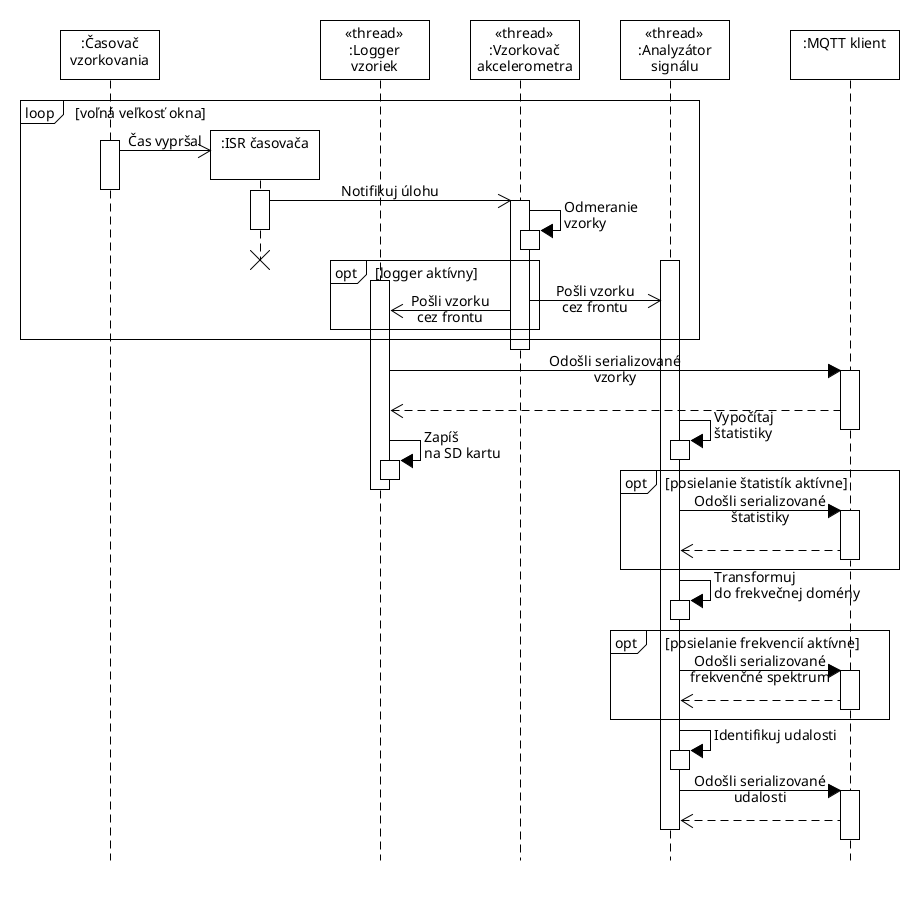
\includegraphics[width=0.9\textwidth]{figures/design/tasks.png}
	\caption{Sekvenčný diagram vzorkovania signálu a spolupráce úloh}
	\label{uml:sequence}
\end{figure}

\section{Etapy spracovania dát}
Poskladané etapy spracovania sa sústredia primárne na odhalenie pretrvávajúcich spektrálnych zložiek. Úloha jednotlivých
zakomponovaných blokov spočíva v prevedení pôvodne obdržaných vzoriek podľa globálnych pravidiel definujúcich ich správanie.

Vo všeobecnosti sa v nej nachádzajú bloky filtrácie, transformácie a serializácie signálu. Sústava sa
vyznačuje modulárnosťou, čiže umožňuje doplnenie dodatočných etáp, ale iba v jednej na seba nadväzujúcej
línii naraz, so spoločnou veľkosťou posuvného okna. Diagram aktivít \ref{pipeline}
vizualizuje navrhovaný beh činností na zariadení.

\subsection{Nastaviteľné vlastnosti}
Utváranie charakteru výstupov sa deje hneď na začiatku voľbou nastavení snímača.
Vzťahuje sa naň vzorkovacia frekvencia časovača, podmieňujúca výstupný dátový tok konštrukčne obmedzený do 952 Hz,
a dynamický rozsah v rozmedzí do 16 $g$. Keďže sú priestorové osi zrýchlenia analyzované nezávisle, vyžadujú sa pre každú ďalšiu
dimenziu systémové prostriedky navyše. Preto je výhodná možnosť aktivácia len niektorých osí.

Postupnosť hodnôt je rozkúskovaná podľa dĺžky vyrovnávacej pamäte pre prevod do frekvenčnej domény s počtom slotov
o mocnine dvojky. Pomer prekryvu okien sa odporúča od 0, čo znamená bez zanechania predošlého obsahu, nanajvýš
do 0,75 výhradne pre úzke oknové funkcie.

Po naplnení miest v cyklickom rade sa pristúpi k prenásobeniu bodov s koeficientami oknovej funkcie
z ponuky: obdĺžnik, Bartlett, Hann, Hamming, Blackman, a následnej Fourierovej alebo kosínusovej transformácii
o veľkosti totožnej s dĺžkou okna. Z frekvenčných vedierok sa zistí magnitúda v lineárnej alebo decibelovej škále.
Pred a po transformácii sa môže doplnkovo uplatniť filter vyhladzovania priemerom, v časovej i vo frekvenčnej doméne.
Opierajú sa o predpísanú veľkosť masky filtra a počet prechodov koľkokrát má byť opakovane aplikovaný.

Identifikácia udalostí pozostáva z binárnej klasifikácie úrovní frekvenčných vedierok podľa prítomnosti lokálneho maxima a
zo zlúčenia súvislého výskytu naprieč dlhším časovým intervalom do udalosti. Klasifikácia sa realizuje
aktuálne nastaveným algoritmom na hľadanie špičiek podľa kombinácie potrebných číselných parametrov. K dispozícii sú
algoritmy: nad prahovú úroveň, najvyššieho spomedzi susedov, prechodu nulou do záporu alebo horského turistu.

\begin{figure}[h!]
	\centering
	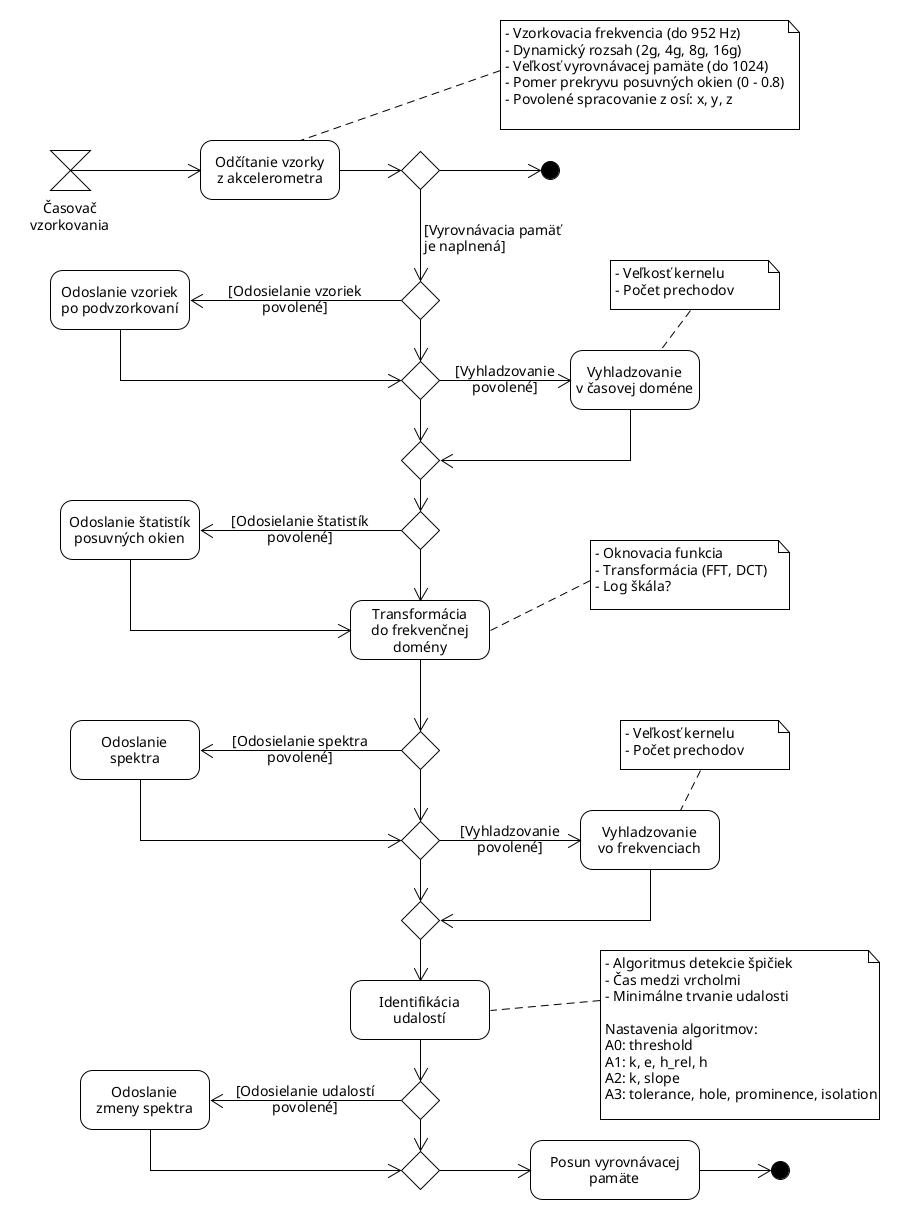
\includegraphics[width=\textwidth]{figures/design/pipeline.png}
	\caption{Postup spracovania zaznamenávaných vibrácií}
	\label{pipeline}
\end{figure}

Medzi dôležitými fázami spracovania dochádza podľa povolených modulov na odosielanie správ k odovzdaniu medziproduktov na formátovanie
cez Message Pack a synchrónne publikovanie na MQTT tému. Umožňuje sa poslanie vzoriek po decimácii celočíselným faktorom $\geq 1$,
požadovaných štatistík z časového priebehu (minimum, maximum, stredná kvadratická odchýlka, priemer, rozptyl, smerodajná odchýlka,
šikmosť, špicatosť, medián, mediánová absolútna odchýlka, medzi-osová korelácia), výsledku frekvenčnej transformácie alebo udalostí
o zmene významných frekvencií.

Reguláciu toku dát a vlastnosti úpravy v etapách spracovania dát ovplyvňuje globálna systémová konfigurácia. Obvykle sa nahrá
z nevolatilnej pamäte, ale je umožnené, aby pravidlá boli upraviteľné vzdialene správami vo formáte Message Pack (\ref{config-change}).
Zariadenie sa prihlási na odber MQTT témy na zmenu konfigurácie. Postačuje, aby na tému klient odoslal vlastnosti, ktoré mieni
upraviť. Ak sú parametre syntakticky korektné a spadajú do dovoleného číselného intervalu príde k reštartu zariadenia a ich
následnému uplatneniu. V opačnom prípade sa na samostatnú MQTT tému odošle chybová hláška.

Vzdialený klient si taktiež dokáže zobraziť všetky momentálne platné pravidlá odberom témy \emph{config/request} a publikovaním na tému
\emph{config/response}, čím sa imituje query-driven vzor požiadavka -- odpoveď.

\begin{figure}[h]
	\centering
	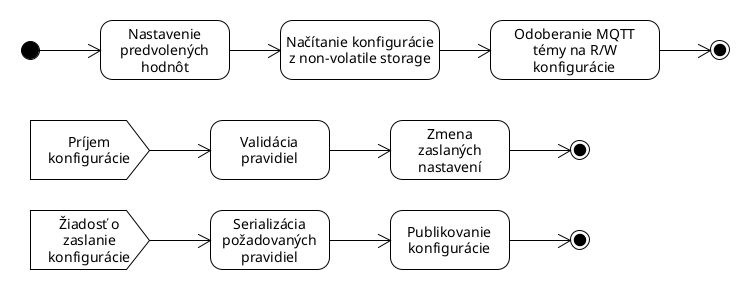
\includegraphics[width=0.9\textwidth]{figures/design/configuration.png}
	\caption{Príjem nových pravidiel a dopytovanie systémovej konfigurácie}
	\label{config-change}
\end{figure}

\subsection{Preskúmané obmeny postupu spracovania}
Uvažovalo sa o vložení voliteľného kroku zníženia šumu v transformovanom spektre Welchovou metódou, ktorý by vedel prispieť
k eliminácii záchvevov krátkodobého výpadku frekvenčnej zložky. Nespolupracuje však dobre s ideou zdieľanej veľkosti okna a
ich prekryvu. Vo všestrannom riešení môžu byť body delené do viacerých segmentov, čo naráža na pamäťové obmedzenia zariadenia
pri viacerých alebo dlhších segmentoch. Zároveň sa znižuje presnosť v časovej oblasti, ktorú by bolo potrebné zohľadniť v časových
pečiatkach udalostí.

Exploratívnou analýzou sa preukázalo, že v uvažovanom kontexte dopravy nemá zmysel extrahovať zo snímaného zrýchlenia odhad
o rýchlosti a polohe numerickou kvadratúrou korigovanou obálkami, respektíve pre vysoký šum sú úrovne veličín nerealistické.
Korekcia má opodstatnenie iba pre stacionárne signály vytrácajúce sa v situáciach, keď sa os akcelerácie odchýli medzi
rovnovážnymi bodmi, napríklad auto zastavené na svahu.

\subsection{Prúdový algoritmus detekcie zmien frekvencií}
Detekcia špičiek sa vzťahuje na frekvenčné spektrum práve prebiehajúceho posuvného okna, čím postráda širší pohľad na trvácnosť
harmonických zložiek v časovo-frekvenčnom priebehu. Okrem toho prirodzene dochádza k dočasným výpadkom v intenzite frekvenčného
vedierka, či už skutočným prerušením, výkyvom do vedľajších vedierok, alebo spôsobeného nespoľahlivosťou označenia lokálnych extrémov.
Všetko sú to javy, ktoré je žiaduce potlačiť v tolerovaných medziach. Doteraz videné body nie je akceptovateľné odložiť v svojej
celistvosti, či úplnosti, aj s ohľadom na promptné ohlásenie udalostí.
\begin{figure}[h!]
\centering
\begin{subfigure}[b]{0.8\textwidth}
    \centering
    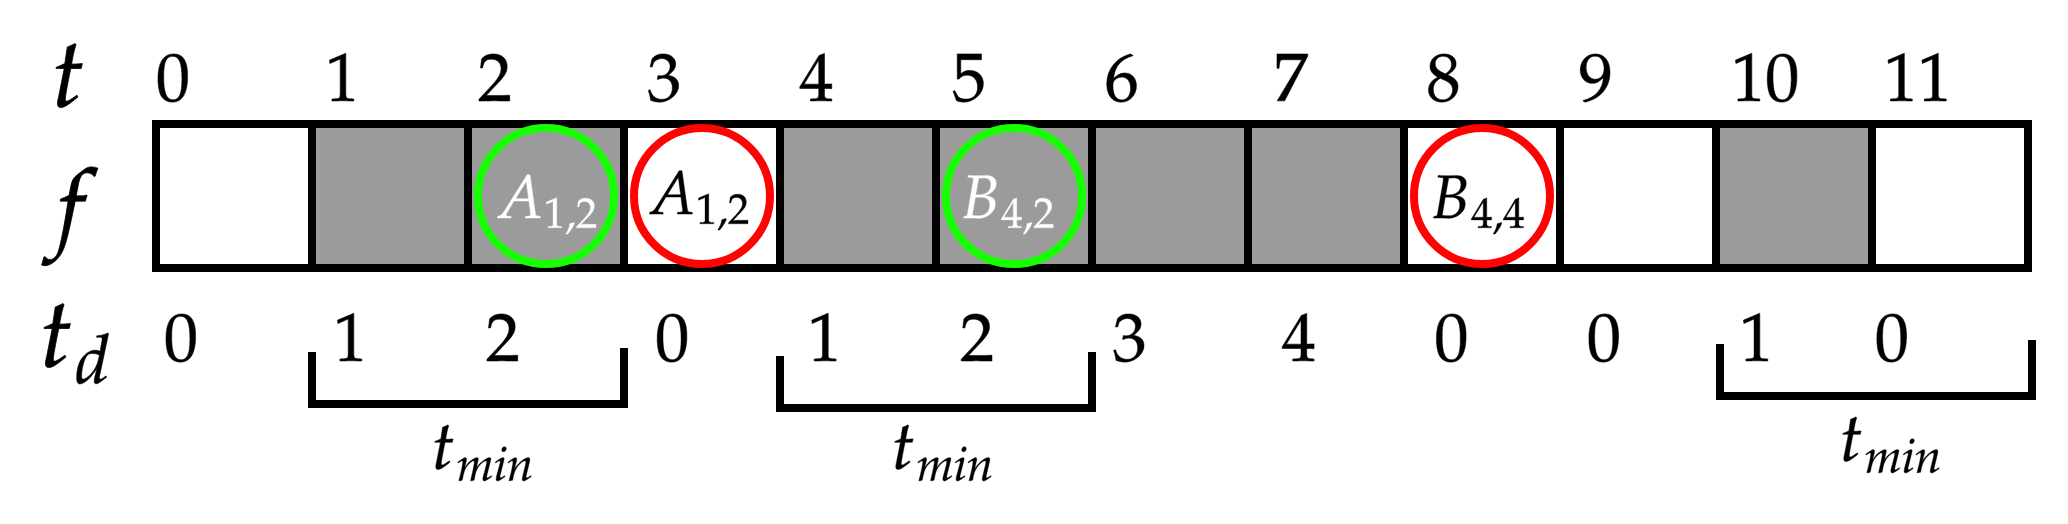
\includegraphics[width=\textwidth]{figures/design/event-detection-min-duration.png}
    \caption{Minimálne trvanie udalosti $t_{min} = 2$}
    \label{event-detector:tmin}
\end{subfigure}
\begin{subfigure}[b]{0.8\textwidth}
    \centering
    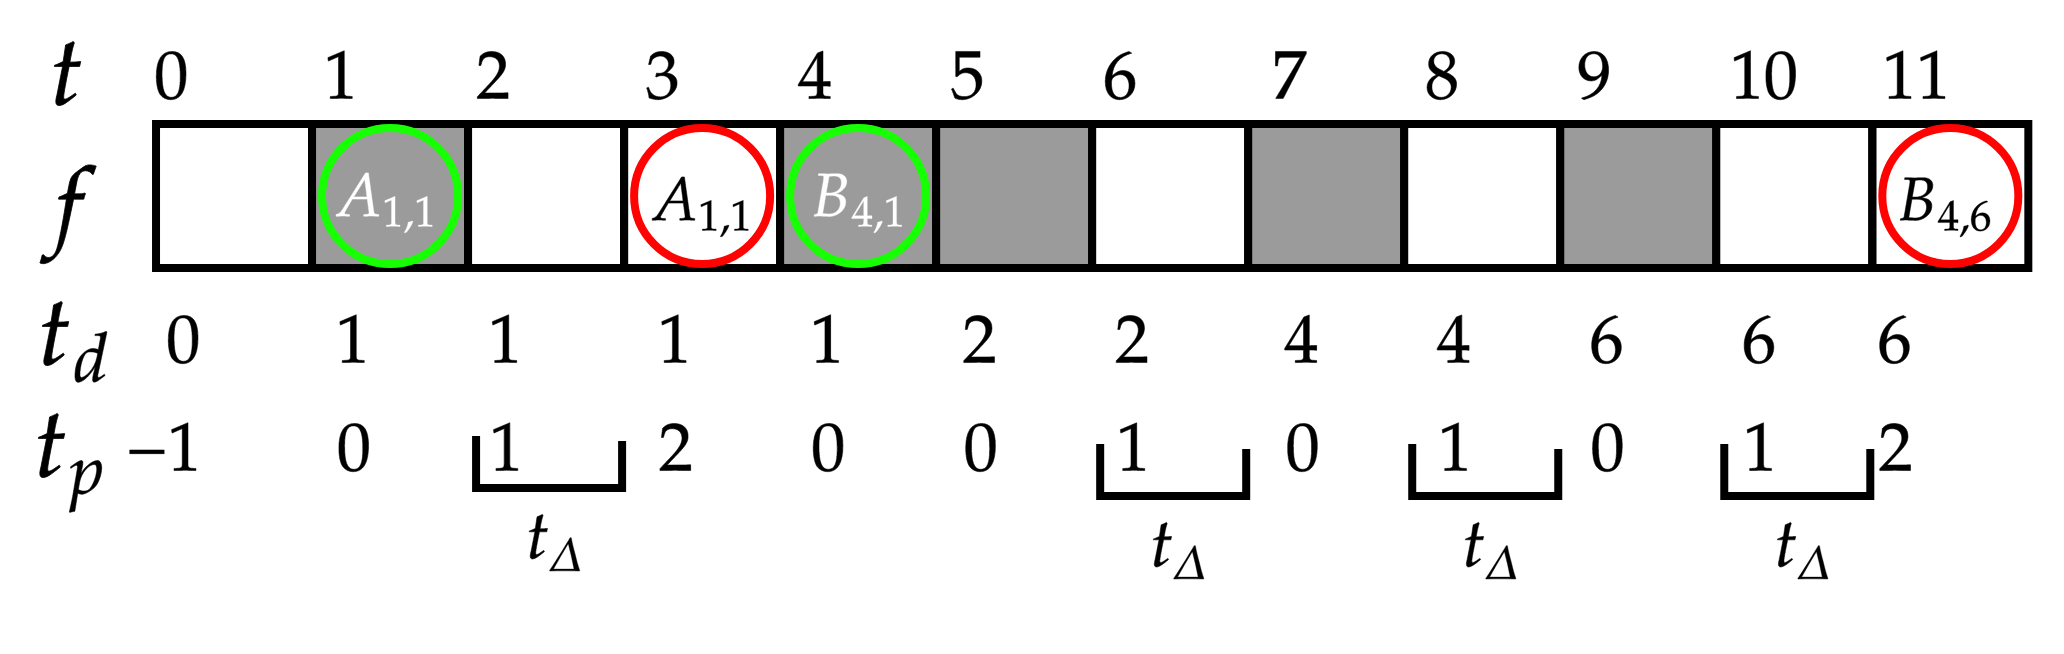
\includegraphics[width=\textwidth]{figures/design/event-detection-time-proximity.png}
    \caption{Maximálna vzdialenosť špičiek $t_{\Delta} = 1$}
     \label{event-detector:tdelta}
\end{subfigure}
\caption{Parametre algoritmu na detekciu udalostí}
\label{event-detector}
\end{figure}

Vývoj detegovaných vrcholov v diskrétnej frekvencii sa dá znázorniť ako binárna sekvencia, kedy prítomnosť vrchola na časovom úseku
označíme logickou jednotkou, na obr. \ref{event-detector} tieňované šedou farbou. Zavedieme dve premenné definujúce aká postupnosť
detekcií klasifikátora špičiek je považovaná za súvislú udalosť.

Parameter $t_{min}$ je najkratšie akceptovateľné trvanie udalosti a predurčuje oneskorenie notifikácie od počiatku objavenia sa zreteľne
vyčlenenej magnitúdy. Čas $t_{\Delta}$ je najdlhšia medzera medzi špičkami tak, aby pretrvávajúca udalosť nebola pri zákmite ukončená alebo
príliš krátka zahodená, ale hluché miesto sa má preklenúť. Tiež vplýva na omeškanie upozornenia na záver udalosti.
Obe premenné sú celočíselné a uvádzajú sa v počte posuvných okien. Najjednoduchší prípad, kedy je udalosťou
neprerušovaná postupnosť jedničiek platí pri $t_{min} = 1$ a $t_{\Delta} = 0$.
\begin{algorithm}[h]
\caption{Detektor zmeny frekvenčnej zložky}
\begin{algorithmic}[1]
\Require{$event$, $bin$, $t$, $t_{min}$, $t_{\Delta}$}
\If {V predošlom okne $t - 1$ bola emitovaná udalosť Koniec}
	\State Vynuluj udalosť: $event$: $duration \gets amplitude \gets 0$, $lastSeen \gets -1$
\EndIf

\If {$\mathrm{IsPeak}(bin)$}
	\State $link \gets \max\{1, event.lastSeen + 1\}$
	\If {$event.duration < t_{min} \leq event.duration + link$}
		\State $event.start \gets t - event.duration - link + 1$
		\State \textbf{Emituj udalosť Štart} výskytu frekvencie podľa $event$
	\EndIf

	\State \textbf{Inkrementuj} $event.duration$ \textbf{o} $link$
	\State \textbf{Inkrementuj} $event.amplitude$ \textbf{o} $(bin - event.amplitude)\;/\;event.duration$
	\State $event.lastSeen \gets 0$

\ElsIf {$event.lastSeen \geq 0$}
	\State \textbf{Inkrementuj} $event.lastSeen$ \textbf{o}  $1$

	\If {$event.lastSeen > t_{\Delta}$}
        	\If {$event.duration \geq t_{min}$}
        		\State \textbf{Emituj udalosť Koniec} výskytu frekvencie podľa $event$
        	\EndIf
        \Else
        	\State Vynuluj udalosť: $event$: $duration \gets amplitude \gets 0$, $lastSeen \gets -1$
        \EndIf
\EndIf
\end{algorithmic}
\label{algo:event-detector}
\end{algorithm}

S rastom $t_{min}$ sa udalosť $A$, začínajúca v posuvnom okne s poradovým číslom
$t = 1$, emituje (zelený kruh) až o $t_{min} - 1$ políčok neskôr (\ref{event-detector:tmin}).
Značka konca (červený kruh) je vytvorená ihneď s ukončením súvislého radu špičiek. Krátke udalosti, napr. s eventuálnym štartom
v čase $t = 10$, sú takto ignorované. Dolný index označenia udalosti sa skladá z dvoch čísel: čas začiatku udalosti a jeho predbežné
trvanie: $A_{t,t_d}$.

Za udalosť $B$ sa zvyšovaním $t_{\Delta}$ považuje podľa \ref{event-detector:tdelta} celý úsek od $t = 4$ s trvaním $t_d = 6$.
Premennou $t_p$ sa sleduje koľko miest do minulosti bola naposledy
zistená jednička, za predpokladu neukončenej udalosti. Po inicializácii alebo prekročením hranice preskočiteľného
rozostupu: $t_p > t_{Delta} + 1$, sa musí $t_p$ rovnať $-1$. Priemerná amplitúda frekvencie sa počíta ako bežiaci priemer.

\section{Datasety}
Úspešnosť klasifikácie odhadneme pomocou syntézy digitálneho časového radu so pseudonáhodným spektrálnym profilom.
Vhodnosť navrhovaných metód detekcie udalostí vo frekvenčnej doméne posúdime podľa nameraných vibrácií z reálnej
premávky električiek a autobusov mestskej hromadnej dopravy.

\subsection{Syntéza časovo-premenného spektrálneho profilu}
Exaktná manuálna anotácia vibračného záznamu je úmorný proces vedúci k nejednoznačným rozhodnutiam, ktoré vrcholy považovať
za postačujúco vyčlenené od ostatných bodov. Kontrola presnosti sa však spolieha na zdroj pravdy výskytov harmonických
komponentov.

Vygenerovaním predpisu rozmiestníme náhodnú sadu istého počtu frekvencií, s hodnotami do polovice
definovanej vzorkovacej frekvencie. Celkové trvanie časového radu arbitrárne rozparcelujeme na desať úsekov, pričom
na každom segmente vymedzíme posun začiatku a konca, pre všetky frekvenčné zložky zo sady, náhodne až do dvoch pozícií
vzad alebo vpred. Amplitúdy sa zvolia z rozsahu 0,2 až 2 jednotky.

\myequations{Rovnica periodického kmitania}
\begin{ceqn}\begin{align}
y = y_{max} \cdot \sin(2\pi f \cdot T_s \cdot i); \quad \forall i \in \mathbb{N} \land i \leq f_s t_d \label{eq:sinusoid}
\end{align}\end{ceqn}

\begin{figure}[h]
   \centering
    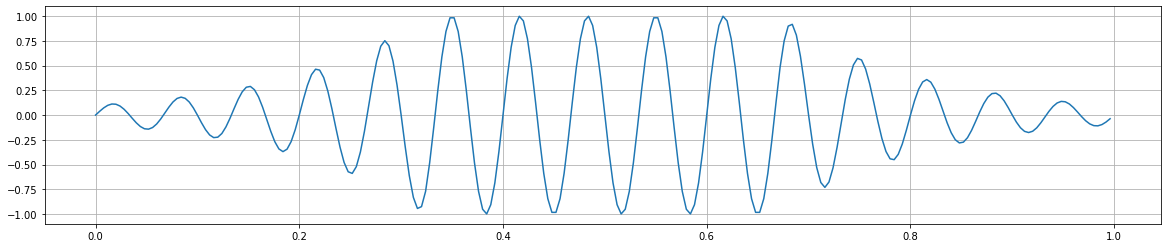
\includegraphics[width=0.9\textwidth]{figures/verification/fade-in-sinusoid.png}
   \caption{Základný tón v syntetickom signále}
   \label{tone}
\end{figure}

Diskrétne sinusoidy s exponenciálnym nábehom amplitúdy (obr. \ref{tone}) mixujeme do postupne zlučovaného vlnového priebehu
podľa pripraveného zoznamu pravidiel. Nábeh a dobeh ovplyvňujú tretinu dĺžky vlny. Vzorky základného tónu s trvaním $t_d$
sú počítané z rovnice periodickej oscilácie (\ref{eq:sinusoid}), kde $i$-ty bod v poradí formuje očakávaná frekvencia $f$
za vzorkovacej periódy $T_s$ a maximálnej amplitúdy $y_{max}$. Skutočné signály postihujú neurčitosti, ktoré napodobíme
pridaním normálne rozdeleného bieleho šumu s úrovňou do 0,1 jednotiek.

Označkovanie aktivity vo frekvenčných vedierkach vznikne rovnako z generovaných deklarácií rozloženia frekvencií
v intervaloch posuvných okien.

\subsection{Zber vibrácií z premávky}
Verný obraz o silách pôsobiacich na prevážané predmety nadobudneme meraniami priamo v doprave.
Umiestnením snímača na podlahu v kabíne pre cestujúcich v blízkosti nápravy alebo nad motorom zachytíme
otrasy najzreteľnejšie.

Záznam ukladaný na pamäťovú kartu spustíme pripojením napájania odporom zaťaženej power banky.
Do novovytvoreného textového súboru sa zapíšu trojrozmerné súradnice vektora zrýchlenia v $m/s^2$ oddelené medzerami
s presnosťou na 3 desatinné miesta. Os $x$ je orientovaná proti smeru jazdy, os $y$ mieri doľava, čo predurčuje smer
osi $z$ dohora. Dynamický rozsah akcelerometra 2 g sa odvodil z prieskumných meraní aplikáciou na mobilnom telefóne.

Na riadkoch súboru sú desatinné čísla so znamienkom do $\pm 20$ prevažne 6 miestne, čím dosiahne jeden záznam súradníc
dĺžku do 21 znakov. OpenLog stíha zapisovať pri 115 000 baud, jednom štart a stop bite na slabiku, teoreticky do
vzorkovacej frekvencie 547 Hz. Pri zachovaní rezervy limitujeme záznam na 500 Hz.
